\documentclass[aspectratio=169]{beamer}
\usetheme[language=ngerman,
titlepagelogo=logopolito,
bullet=circle,
pageofpages=of,
titleline=true,
color=blue
]{TorinoTh}

%\usepackage[ngerman]{babel}
%\usepackage[utf8]{inputenc}
\usepackage{tabularx}
\usepackage{booktabs}
\usepackage{multicol}
\usepackage{ulem}
\usepackage{makecell}
\usepackage{upgreek}
\usepackage{movie15}

\addto{\captionsngerman}{%
  \renewcommand*{\contentsname}{Contents}
  \renewcommand*{\listfigurename}{Figures}
  \renewcommand*{\listtablename}{Tables}
  \renewcommand*{\figurename}{Fig.}	
  \renewcommand*{\tablename}{Tab.}
}

\newcommand{\tabitem}{~~\llap{\textbullet}~~}

\usepackage{color}
\usepackage{graphicx}
\usepackage{fancybox}

\usepackage{beamerthemesplit}
\usetheme[compress]{Heidelberg}
\definecolor{unirot}{rgb}{0.4,0.4,0.3} % babyblue 0,0.58,1
\usecolortheme[named=unirot]{structure}
%\setbeamercolor{alerted text}{fg=red}
\newcommand*\hilite[1]{\textcolor{red}{#1}}
%\def\hilite<#1>{%
  %\temporal<#1>{\color{black}}{\color{unirot}}%
               %{\color{gray}}}

\title[Light Transport Techniques for Tensor Field Visualization]{Light Transport Techniques for Tensor Field Visualization}
%\subtitle{}
\author[Sebastian Bek]{Sebastian Bek}
\date{\today}
\institute[Uni HD]{
Heidelberg University\\
Visual Computing Group (VCG)\\
Master's Thesis Presentation\\
Supervisors: Prof. Filip Sadlo, Dr. Susanne Krömker\\
%\color{unirot}{sebibek@gmail.com}}
}

%---------------------------------------%
%---------- RECURRING OUTLINE ----------%
% have this if you'd like a recurring outline
\AtBeginSection[]  % "Beamer, do the following at the start of every section"
{
\begin{frame}<beamer> 
\frametitle{Outline} % make a frame titled "Outline"
\tableofcontents[currentsection,hideallsubsections]  % show TOC and highlight current section
\end{frame}
}
%----------------------------------------


\begin{document}
\frame[plain]{\titlepage}
\frame{\frametitle{Outline}\tableofcontents[hideallsubsections]}

%========================================
%========================================

\section[Introduction]{Introduction}

\subsection[Introduction]{Motivation}

\frame{
\frametitle{{Motivation}}

\begin{itemize}
	\item visualization in general is needed to generate a more readable, explorable and intuitive representation
	\item tensor representations are needed to describe a directional distribution for each point in space, when:
	\begin{itemize}
	\item e.g. for vector fields: to describe the directionally dependent spatial gradient called Jacobian-matrix,
	\item e.g. for fluid and solid continuum mechanics: to describe a whole distribution of stresses
	\item e.g. for DT-MRI: diffusion tensor - magnetic resonance imaging: to describe the diffusion characteristics of water molecules within tissue
	\end{itemize}
\end{itemize}
} % END OF FRAME


\frame{
\frametitle{{Objectives}}

\begin{itemize}
	\item a light transport model (propagation scheme) following basic but crucial physical principles,
	\item application of this model for tensor field visualization interpreting tensors as light transmission properties,
	\item a FTLE (Finite-time Lyapunov exponents)-related approach called light transport gradient (LTG) for visualizing key structures, namely LCS (Lagrangian coherent structures) in 2D second-order tensor fields, and
	\item application of our approach to both synthetic and real data involving brain and heart datasets.
\end{itemize}

} % END OF FRAME
%----------------------------------------

\subsection[Introduction]{Related Work}

\frame{
\frametitle{{Related Work - Global Illumination Methods}}
\begin{columns}
\begin{column}{.5\textwidth}
\begin{itemize}
	\item Discrete Ordinates Method: discretizes RTE in both spatial and angular domain
	\bigskip
	\item Lattice-Boltzmann method: light propagation modeled as a diffusion process
	\bigskip
	\item Light Propagation Volumes: light exchanged between neighboring cells and stored locally in capacities
\end{itemize}
\end{column}
\begin{column}{.5\textwidth}
\begin{figure}[t]
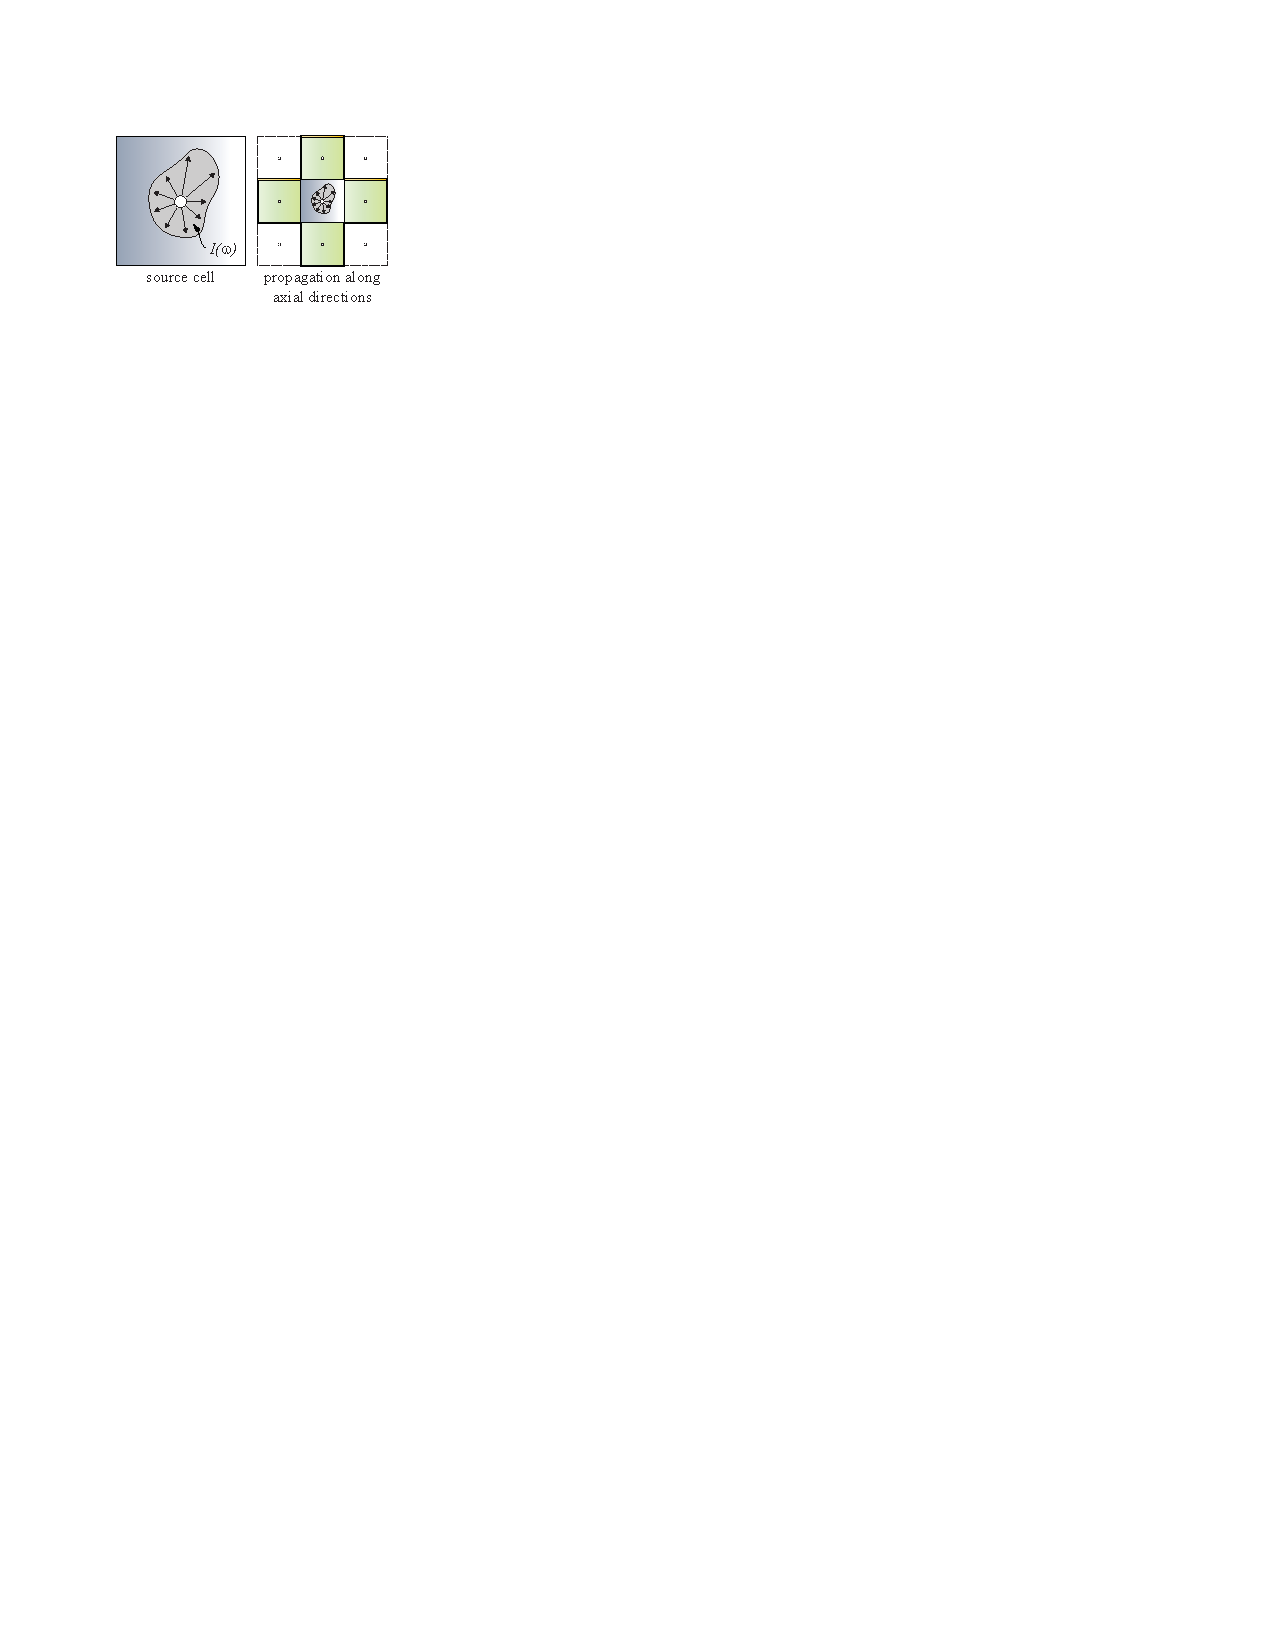
\includegraphics[width=0.5\textwidth]{LPV.pdf} 
\caption{Light Propagation Volumes,  \textit{Source: \textcircled{1}}}
\end{figure}
\end{column}
\end{columns}


} % END OF FRAME

\frame{
\frametitle{{Related Work - Symmetric Tensor Field Visualization}}

\begin{itemize}
	\item Glyphs: represent anisotropy with shape and orientation
	\item Tensor Field Lines (TFLs): follow the eigenvector along tensor field lines
	\item Tensorlines: introduce artificial inertia on TFLs to increase stability
	\item HyperLIC: use Line Integral Convolution from Vector Field Visualization on TFLs
	\item FTLE: exploit the gradient of the flow map of TFLs to generate an FTLE field
	\item Scalar Measures: tensor magnitude, diffusivity, fractional anisotropy, anisotropy coefficients (measures)
\end{itemize}


} % END OF FRAME

\frame{
\frametitle{{Related Work - Asymmetric Tensor Field Visualization}}

\begin{itemize}
	\item Dual Eigenvectors: use complex conjugate eigenvectors as co-visualization for the complex domain along with ordinary eigenvectors to represent the real domain
	\bigskip
	\item Pseudo Eigenvectors: extension for dual eigenvectors to a full set or graph
	\bigskip
	\item Scalar Measures: tensor magnitude, tensor mode, isotropy index
\end{itemize}


} % END OF FRAME
%----------------------------------------


%----------------------------------------

%======================================== END OF SECTION

\section[Fundamentals]{Fundamentals}

\frame{
\frametitle{{Fundamentals}}

\begin{block}{\centering \textbf{Tensor Fields}}
\begin{itemize}
	\item order-$o$ generalization of a matrix with indices of run length $n$ for $n\times n$ matrices
	\item number arrays following covariant or contravariant transformation rules
	\item represenation needed for a whole directional distribution for each point in space
\end{itemize}

\end{block}
\begin{table}[!b]
\centering
\caption{Tensor Shapes}
 \begin{tabular}{c|c|c|c|c|c|c}
\textbf{order} & 0 & 1 & 2 & 3 & ... & o \\ 
\hline 
\textbf{shape} & scalar & vector & matrix & ``3D matrix'' & ... & order-$o$ matrix\\ 
\end{tabular}
\label{tensor}
 \end{table} 
} % END OF FRAME

\frame{
\frametitle{{Fundamentals}}

\begin{columns}
\begin{column}{.5\textwidth}
\begin{block}{\centering \textbf{Cauchy stress tensor}}
\begin{itemize}
	\item classical physical example of a tensor
	\item consistent of $3$ stress vectors arranged in row-major order
	\item these represent the magnitude and orientation of the resulting stress at plane $x,y,z$ in direction $x,y,z$
	\item maps an incoming direction vector $\mathbf{n}$ a resulting stress vector $\mathbf{T^{(n)}} = \mathbf{n}\cdot\boldsymbol{\sigma}$ per transformation
\end{itemize}

\end{block}
\end{column}
\begin{column}{.5\textwidth}
\begin{figure}[t]
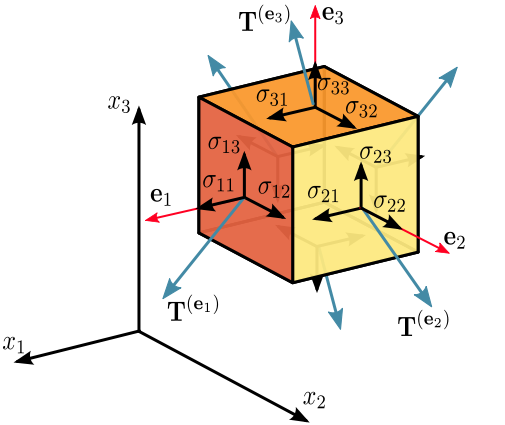
\includegraphics[width=0.5\textwidth]{stress_tensor.png} 
\caption{Cauchy stress tensor,  \textit{Source: \textcircled{2}}}
\end{figure}
\end{column}
\end{columns}

} % END OF FRAME


\frame{
\frametitle{{Polar Coordinates}}

\begin{columns}
\begin{column}{.5\textwidth}
\begin{block}{\centering \textbf{Conversion Formulas}}
Polar$\mapsto$Cartesian
\begin{align*}
	x &= r \cos \omega, \\
 	y &= r \sin \omega.
\end{align*}
Cartesian$\mapsto$Polar
\begin{align*}
	r &= \sqrt{x^2 + y^2}, \\
\omega &= \operatorname{atan2}(y, x).
\end{align*}

\end{block}
\end{column}
\begin{column}{.5\textwidth}
\begin{figure}[t]
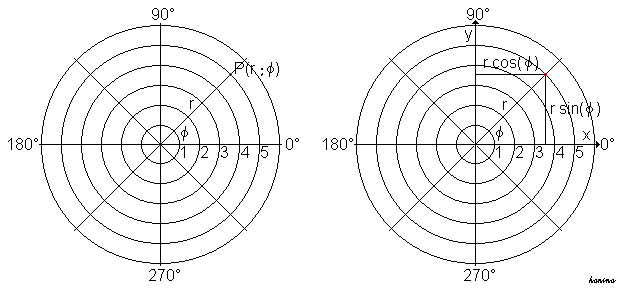
\includegraphics[width=0.7\textwidth]{polarkoordinaten.png}
\caption{Polar coordinates,  \textit{Source: \textcircled{3}}}
\end{figure}
\begin{itemize}
	\item polar function $f: \omega\mapsto r$ maps each angle $\omega$ a magnitude $r(\omega)$
\end{itemize}
\end{column}
\end{columns}

} % END OF FRAME

\frame{
\frametitle{{Principal Component Analysis}}

\begin{columns}
\begin{column}{.6\textwidth}
\begin{small}
\begin{block}{\centering \textbf{Matrix Decompositions}}
Eigenvalue Decomposition: 
$
	\mathbf{A} = \mathbf{R}\mathbf{S}\mathbf{R}^*
$\\
Singular Value Decomposition (SVD): 
$
	\mathbf{A} = \mathbf{U} \mathbf{\Sigma} \mathbf{V}^*
$
\end{block}
\end{small}
\bigskip
\begin{itemize}
	\item used to determine the main directions of variance (principal components) in stochastic data
	\item used to determine the subsequent base transformations composing affine transformations
\end{itemize}

\end{column}
\begin{column}{.4\textwidth}
\begin{figure}[t]
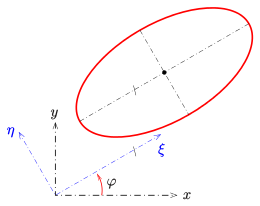
\includegraphics[width=0.7\textwidth]{HAT.png}
\caption{Principal component analysis,  \textit{Source: \textcircled{4}}}
\end{figure}

\end{column}
\end{columns}
} % END OF FRAME


\frame{
\frametitle{{Principal Component Analysis}}


\includemovie{0.49\textwidth}{0.4\textwidth}{scale.swf}
\includemovie{0.49\textwidth}{0.4\textwidth}{rotate.swf}


} % END OF FRAME

\frame{
\frametitle{{Finite-Time Lyapunov exponents}}

\begin{columns}
\begin{column}{.6\textwidth}
\begin{small}
\begin{block}{\centering \textbf{Definition}}
Local: 
$
	\sigma = \frac{1}{\lvert T\rvert}\ln \frac{\Delta}{\delta}
$\\
Global: 
$
	\sigma(\mathbf{x})=\frac{1}{\lvert T\rvert}\ln \|\nabla\mathbf{\upvarphi(x)}\|_2
$\\
{\scriptsize whereas $\| A\| _2 = \sqrt{\lambda_{max}(A^TA)}$ is the spectral norm of matrix $A$}
\end{block}
\end{small}
\begin{itemize}
	\item measure for separation abilities of time-dependent dynamical systems concerning massless tracer particles
	\item in particular concerning Lagrangian view in vector fields: placing two close-by particles into and moving with the flow
\end{itemize}

\end{column}
\begin{column}{.4\textwidth}
\begin{figure}[t]
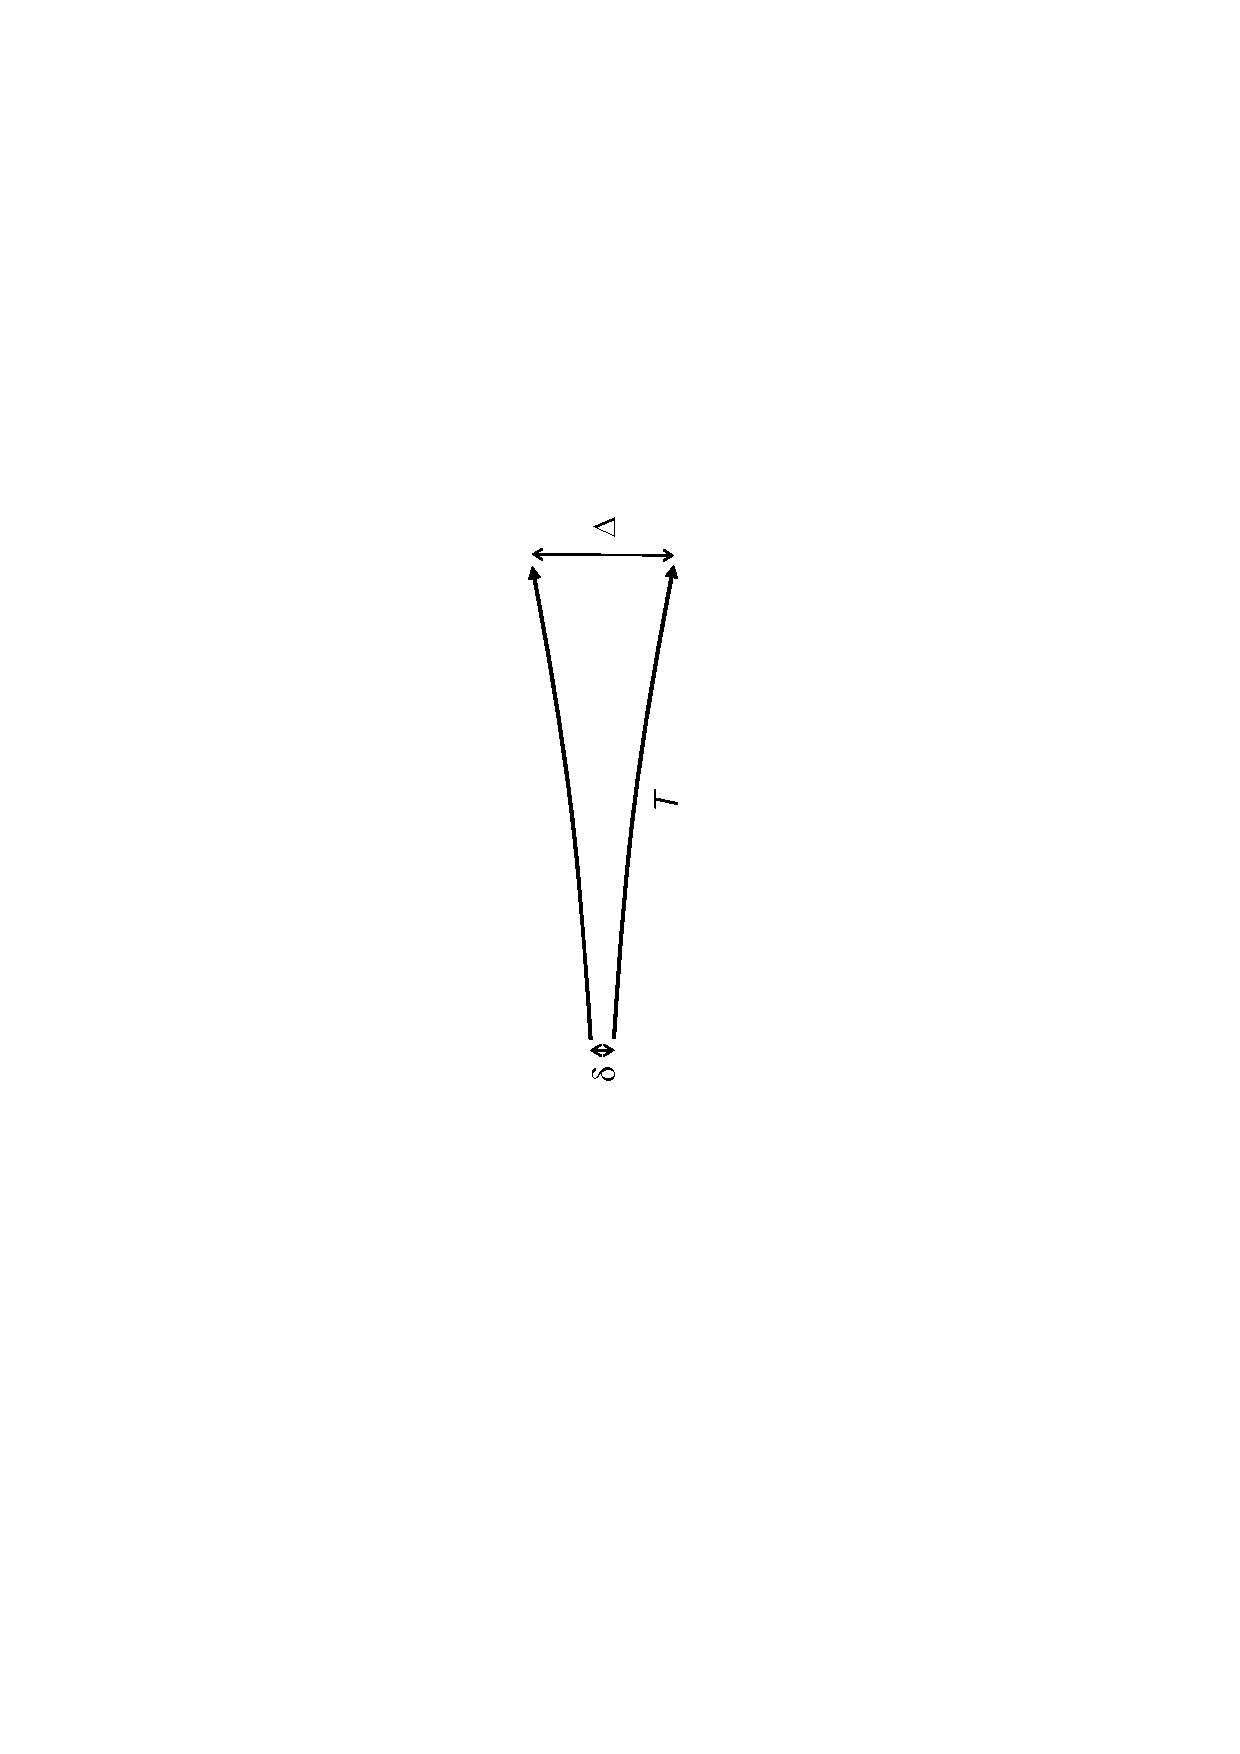
\includegraphics[height=0.9\textwidth]{ftle_sep.pdf}
\caption{Path line separation,  \textit{Source: \textcircled{4}}}
\end{figure}

\end{column}
\end{columns}
} % END OF FRAME

\frame{
\frametitle{{Glyphs}}
\begin{columns}
\begin{column}{.6\textwidth}
\begin{small}
\begin{itemize}
	\item glyphs are used to represent the principal component ellipsoid, i.e., the anisotropy characteristics and/or tensor magnitude
	\bigskip
	\item glyphs can be found in varying shapes, we define ellipsoids here for simplicity
\end{itemize}
\end{small}
\end{column}
\begin{column}{.4\textwidth}
\begin{figure}[t]
\centering
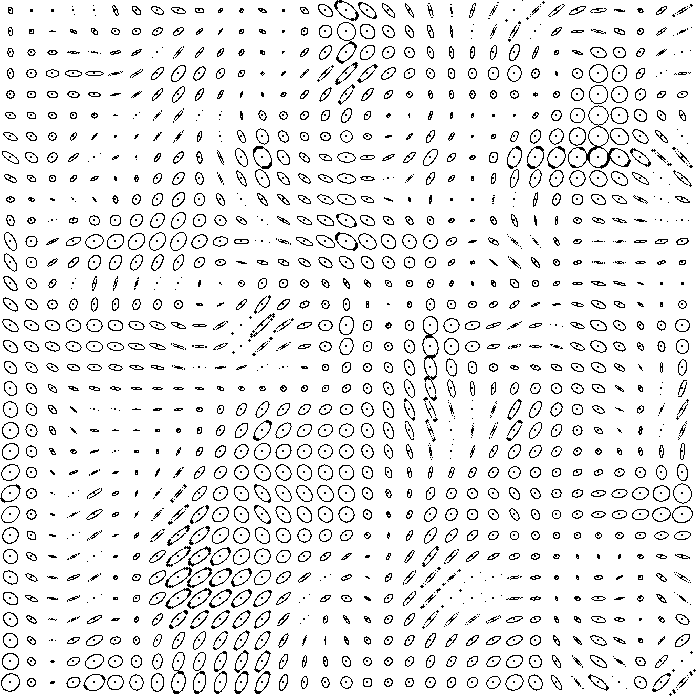
\includegraphics[height=0.9\textwidth]{random-global.png}
\caption{$2D$ glyphs for Random field}
\end{figure}

\end{column}
\end{columns}
} % END OF FRAME

\frame{
\frametitle{{Tensor Field Lines}}

\begin{columns}
\begin{column}{.6\textwidth}
\begin{small}
\begin{block}{\centering \textbf{Procedure}}
follow major/minor eigenvectors along pathlines
\end{block}
\end{small}
\bigskip
\begin{itemize}
	\item ambiguity for nearly isotropic cases: small changes in magnitude effect large changes in glyph orientation
	\item therefore susceptive to noise in data
\end{itemize}

\end{column}
\begin{column}{.4\textwidth}
\begin{figure}[t]
\centering
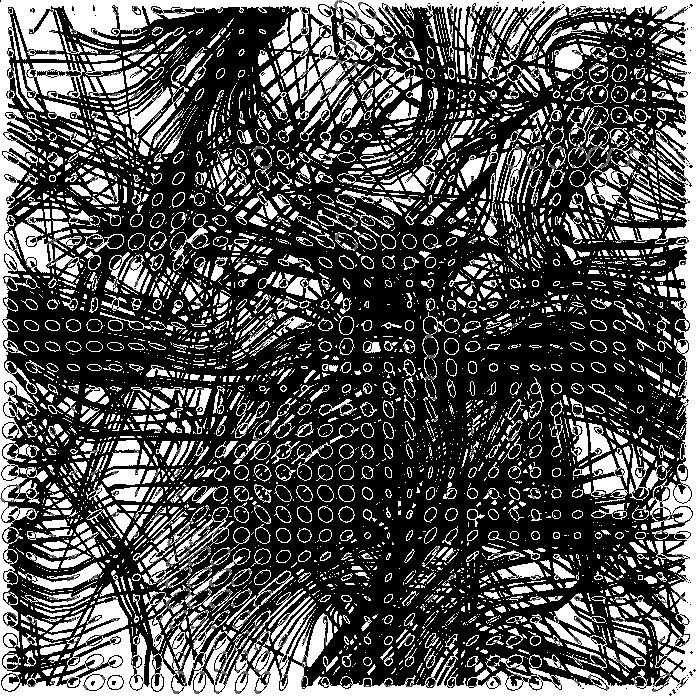
\includegraphics[height=0.9\textwidth]{random-global-TFL.png}
\caption{$2D$ glyphs and tensor field lines}
\end{figure}

\end{column}
\end{columns}
} % END OF FRAME

\frame{
\frametitle{{Asymmetric Tensor Fields}}

\begin{figure}[!t]
\centering
  \begin{minipage}{0.3\textwidth}
      \centering
    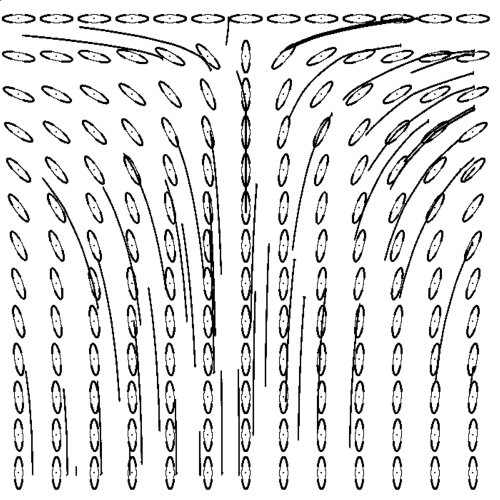
\includegraphics[height=\textwidth]{drain(alt)-TFL.png}
	a)
    \label{a)}
  \end{minipage}
  \begin{minipage}{0.3\textwidth}
      \centering
    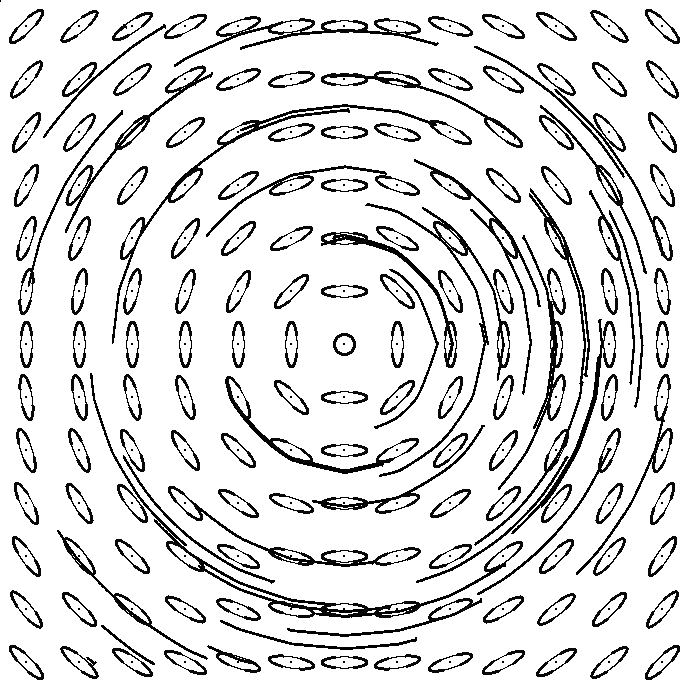
\includegraphics[height=\textwidth]{tensorfieldlines.png}
	b)
    \label{b)}
  \end{minipage}
  \begin{minipage}{0.3\textwidth}
      \centering
    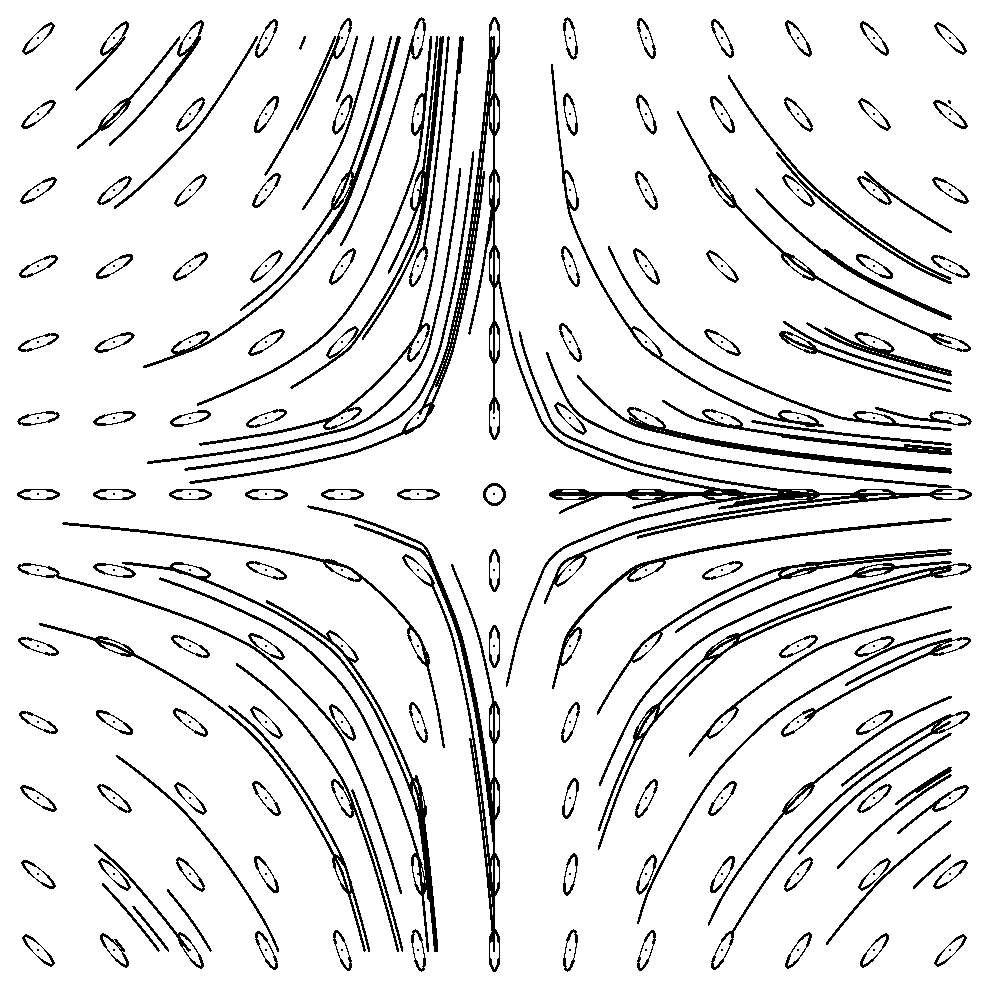
\includegraphics[height=\textwidth]{inverse-TFL.png}
	c)
    \label{b)}
  \end{minipage}
\caption{Several test fields: a)Drain, Rings, Inverse}
\label{test_fields2}
\end{figure}

} % END OF FRAME

\frame{
\frametitle{{Symmetric Tensor Fields}}

\begin{figure}[!t]
\centering
  \begin{minipage}{0.4\textwidth}
    \centering
    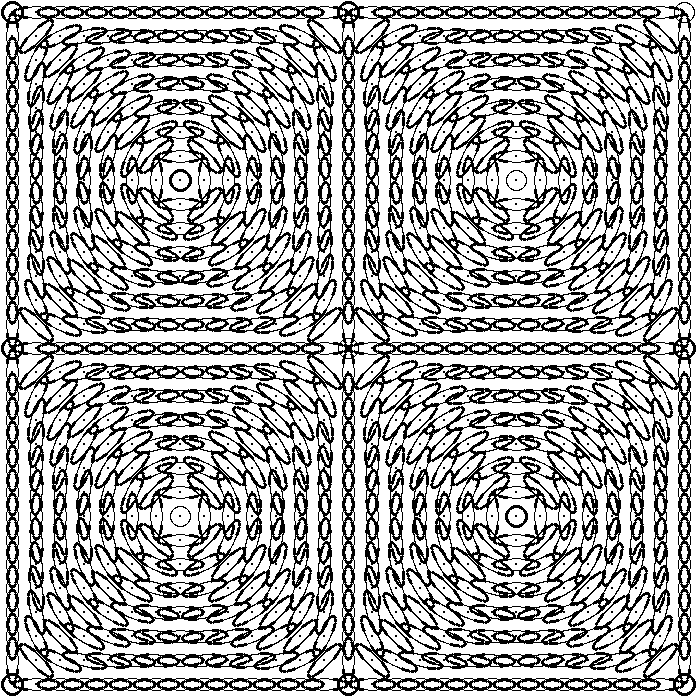
\includegraphics[width=0.8\textwidth]{gyre.png}
	a)
    \label{a)}
  \end{minipage}
  \begin{minipage}{0.4\textwidth}
    \centering
    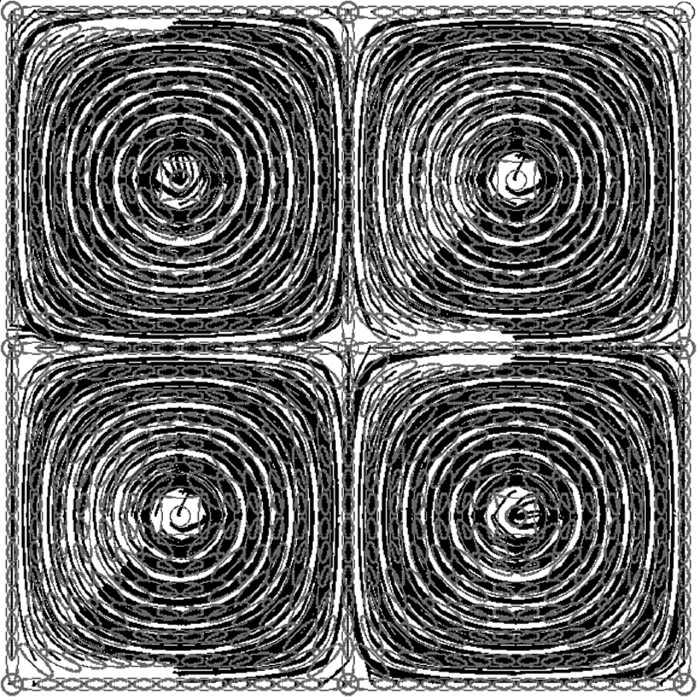
\includegraphics[width=0.8\textwidth]{gyre-TFL.png}
	b)
    \label{b)}
  \end{minipage}
\caption{Gyre test field: a) glyphs, b) tensor field lines for a)}
\label{gyre}
\end{figure}

} % END OF FRAME

\frame{
\frametitle{{Asymmetric Tensor Fields}}

\begin{figure}[!t]
\centering
  \begin{minipage}{0.2\textwidth}
  \centering
    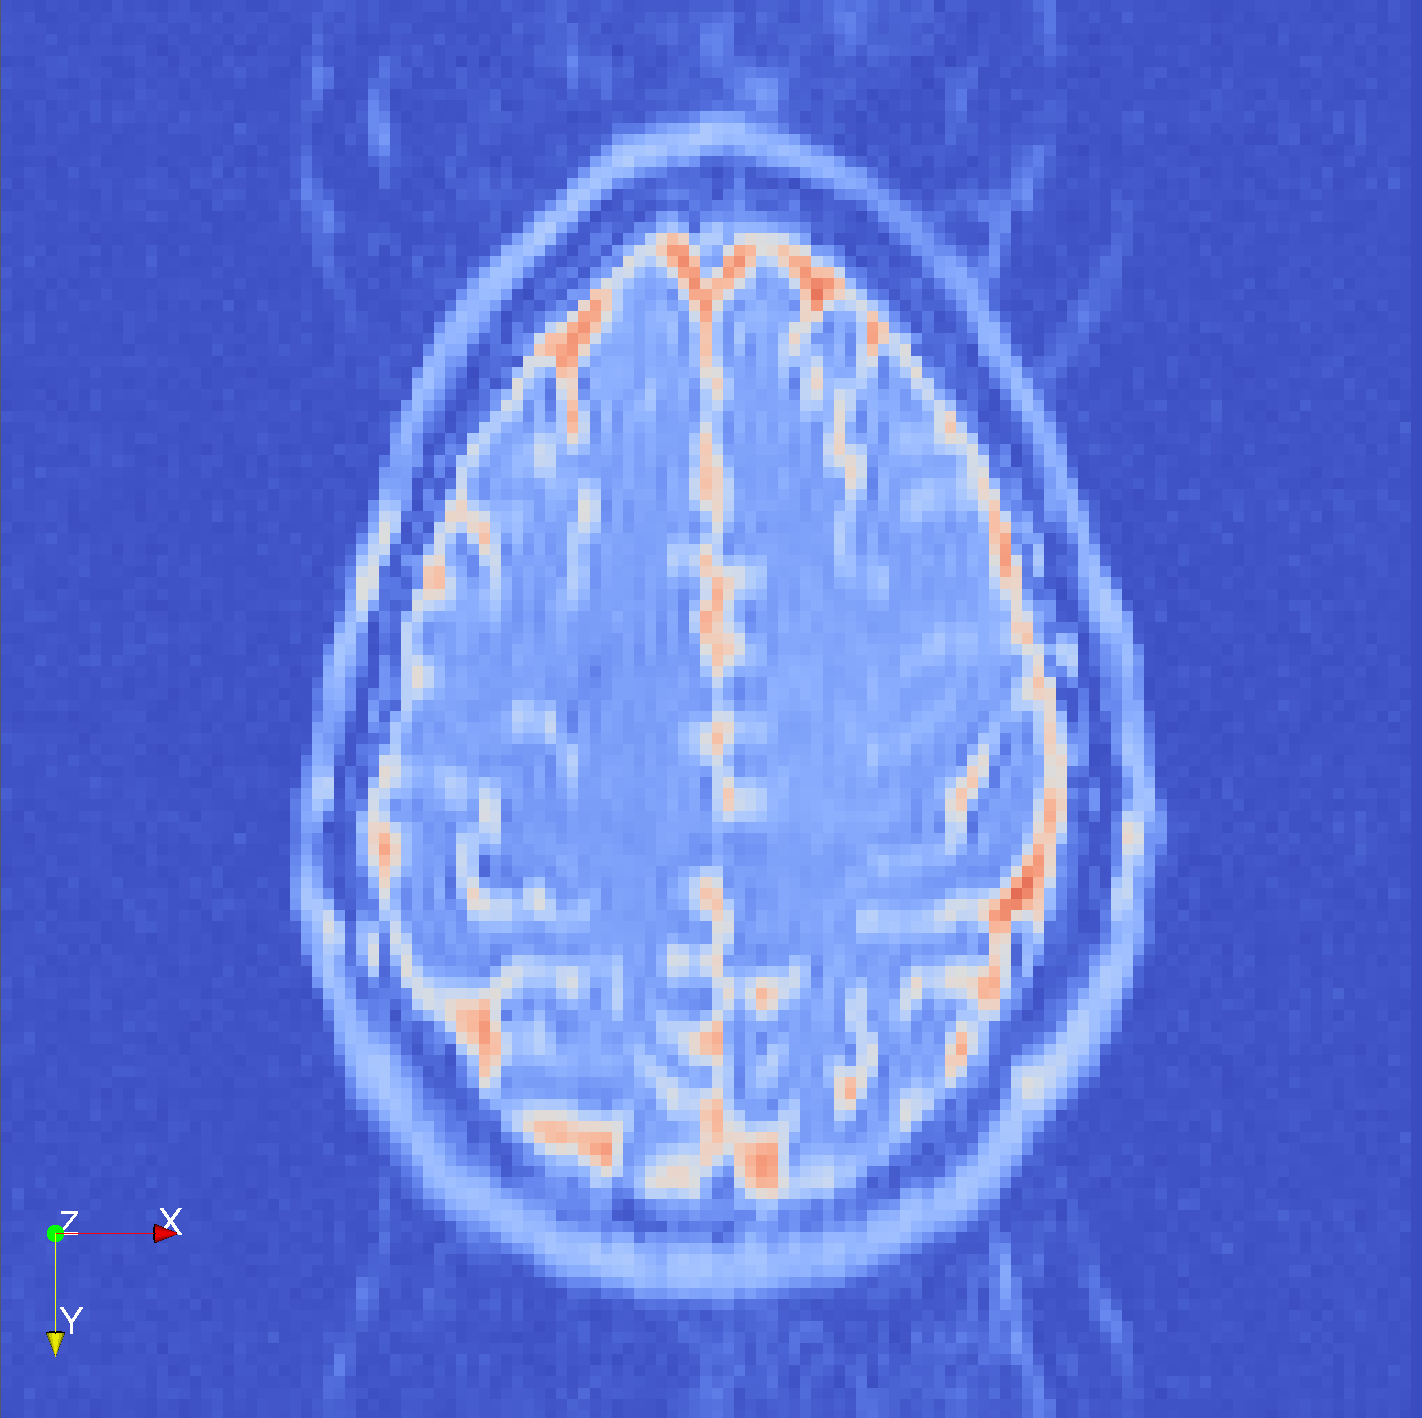
\includegraphics[width=0.8\textwidth]{brain_org.png}
    \label{a)}
	a)
  \end{minipage}
  \begin{minipage}{0.2\textwidth}
  \centering
    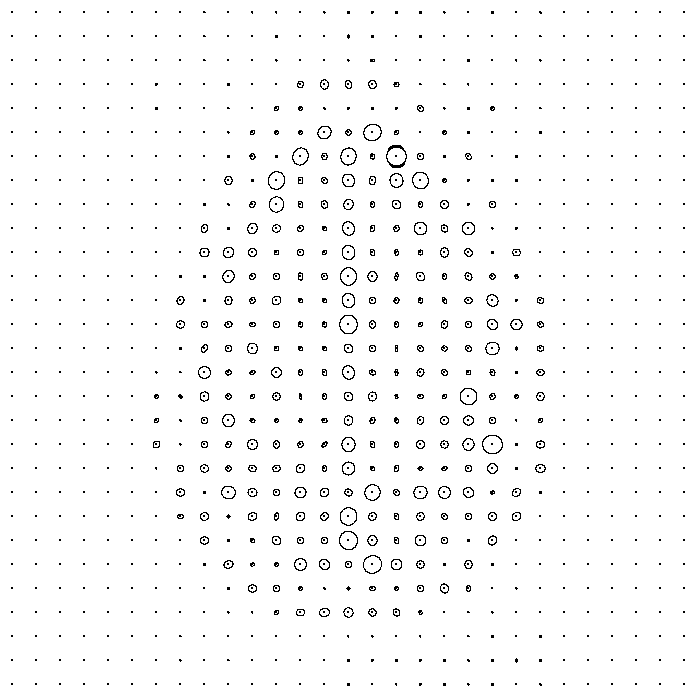
\includegraphics[width=0.8\textwidth]{brainDwnsmpl.png}
    \label{b)}
    b)
  \end{minipage}
  \begin{minipage}{0.2\textwidth}
  \centering
    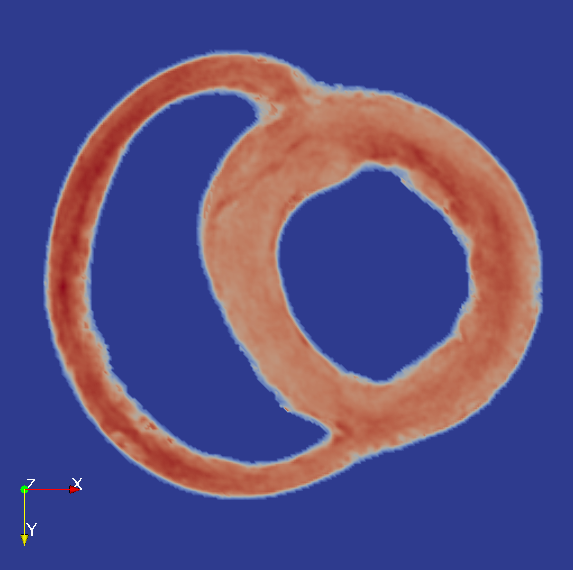
\includegraphics[width=0.8\textwidth]{heart_org.png}
    \label{b)}
    a)
  \end{minipage}
  \begin{minipage}{0.2\textwidth}
  \centering
    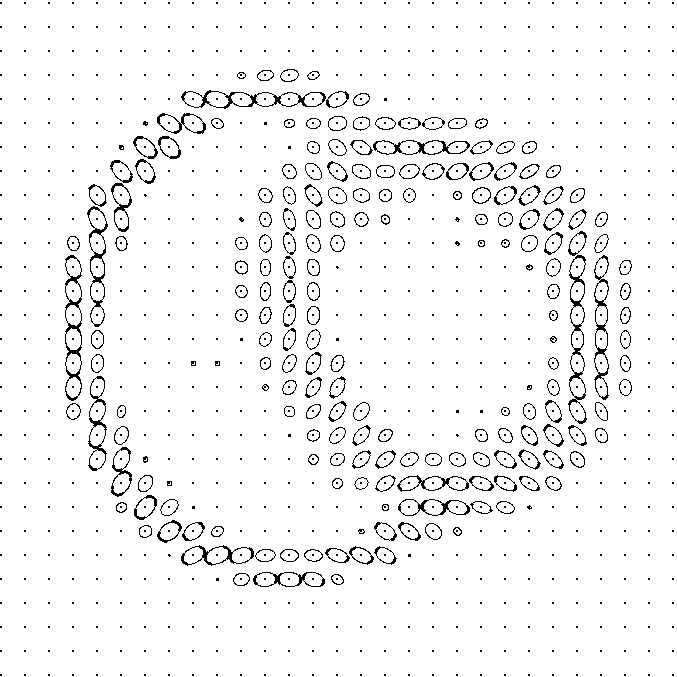
\includegraphics[width=0.8\textwidth]{heartDwnsmpl.png}
    \label{b)}
    b)
  \end{minipage}
\caption{Brain and Heart dataset: a) tensor magnitude, b) ellipsoid glyphs}
\label{real1}
\end{figure}

%\begin{figure}[!t]
%\centering
%  \begin{minipage}{0.2\textwidth}
%    \centering
%    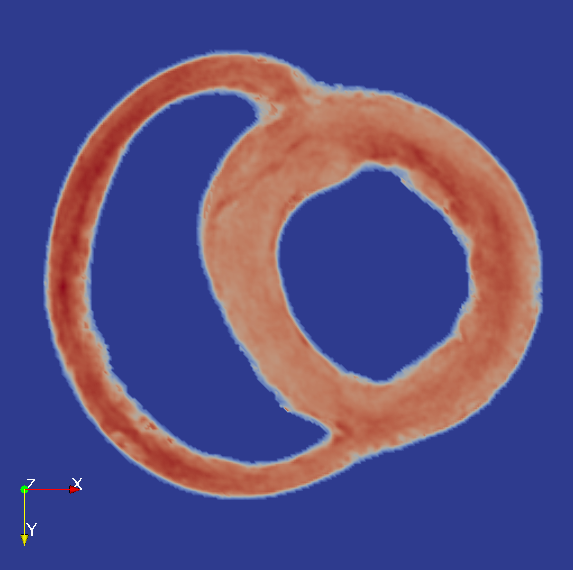
\includegraphics[width=0.8\textwidth]{heart_org.png}
%    \label{a)}
%	a)
%  \end{minipage}
%  \begin{minipage}{0.2\textwidth}
%    \centering
%      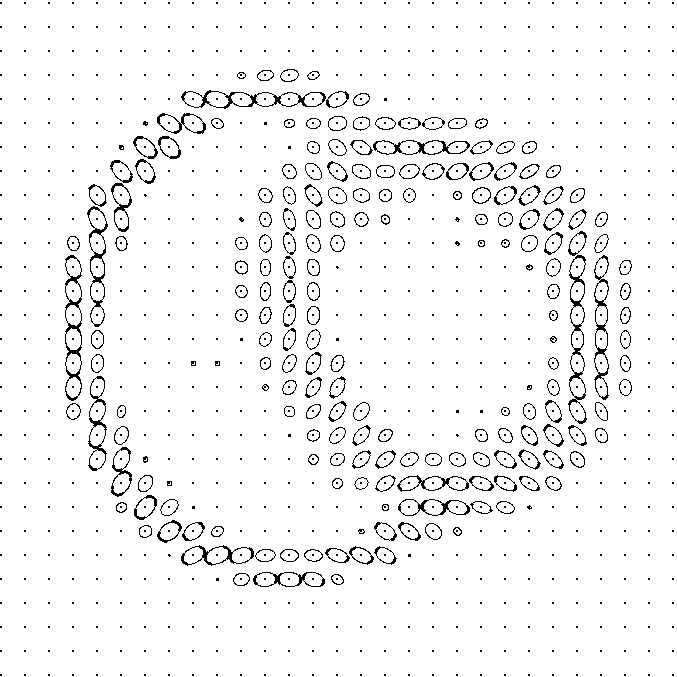
\includegraphics[width=0.8\textwidth]{heartDwnsmpl.png}
%    \label{b)}
%	b)
%  \end{minipage}
%\caption{Heart dataset: a) tensor magnitude, b) ellipsoid glyphs}
%\label{real2}
%\end{figure}

} % END OF FRAME

\section[Method]{Method}


\section[Results and Evaluation]{Results and Evaluation}
%----------------------------------------

%\footnotetext{Goodfellow, Ian, et al. "Generative adversarial nets."}

%----------------------------------------

\section[Conclusion and Future Work]{Conclusion and Future Work}

\frame{
\frametitle{Summary}

\begin{itemize}
\item GANs: new framework for estimating \alert{generative models} defined by multilayer perceptrons (Convolutional Layers) trained by standard backpropagation $\rightarrow$ no need for any Markov chains (MCMC-approaches), which can have problems Mixing (Converging)
\item Results\/ Samples considered to be \alert{competitive} with those of the state-of-the-art generative models
\item Empirical Evaluation (Fitting a Gaussian Parzen window to measure distribution similarity of $p_g$ as log-likelihood metric) indicates comparable scores than achieved for state-of-the-art methods like DBNs, Stacked CAE, GSN, Adversarial nets and \alert{comparable validity/representativity}
\end{itemize}
%\footnotetext{Goodfellow, Ian, et al. "Generative adversarial nets."}
} % END OF FRAME
%----------------------------------------

\frame{
\frametitle{Conclusion}

\begin{itemize}
\item approach is, besides DGMs (directed graphical models), the only one, inducing \alert{no problems} or further elaborations for sampling (generating samples) or training $\rightarrow$ rather simple implementation
\item experiments show \alert{comparable similarities} against state-of-the-art methods in log-likelhood score and variance in matching the prior distribution $p_z$ with the generative one ($p_g$), but the method proposed is regarded to be more simple than others
\item the \alert{synchronization of D} is yet an effortful factor, since sufficient reasoning for the number of steps of the inner loop is needed to avoid the previously named "Helvetica scenario"!
\item \alert{future applications} might involve the synthetic generation of morphologically correct segmentation masks of seperatable objects, fake images (databases), keys/passwords (cryptography), image processing
\end{itemize}

%\footnotetext{Goodfellow, Ian, et al. "Generative adversarial nets."}
} % END OF FRAME
%----------------------------------------

\frame{
\frametitle{Outlook}
\textbf{Straighforward extensions}:
\begin{enumerate}
\item Conditional generative Model $p(\mathbf{x}|c)$ w. adding condition $c$
\item Learned approximate inference: Predict prior-$z$ w. given latent $x$
\item Modeling of multiple Conditionals: $p(\mathbf{x}_S|\mathbf{x}_\xout{S})$
\item Semi-Supervised Learning: Better Performance w. partially labeled training data
\item Efficiency improvements: Better methods to coordinate $G$ and $D$, better distributions to sample $z$ from during training
\end{enumerate}

%\footnotetext{Goodfellow, Ian, et al. "Generative adversarial nets."
} % END OF FRAME
%----------------------------------------

%========================================

%\frame{
%\frametitle{Vor - Nachteile}
%
%\begin{columns}[b]
%\begin{column}{.5\textwidth}
%{\color{unirot}Vorteile}
%\begin{itemize}
%  \item da gibt es viele
%  \item und noch mehr
%  \item und immer mehr
%  \item und ein letzter Vorteil
%\end{itemize}
%\end{column}
%
%
%\begin{column}{.5\textwidth}
%{\color{unirot}Nachteile} 
%\begin{itemize}
%  \item da gibt nur einen
%  \item oder zwei
%\end{itemize}
%\end{column}
%
%\end{columns}
%\vfill
%} % END OF FRAME


%========================================
%========================================
%========================================

% hilights mit \alert oder \hilite




%----------------------------------------

\frame{\frametitle{Questions?}
\begin{figure}

\includegraphics[width=.8\textwidth]{img/questions} 
\end{figure}
\vspace*{-3.3cm}\begin{center}\begin{LARGE}\textbf{Questions?}\end{LARGE}\end{center}

\vspace*{2cm}
}

\frame{
\frametitle{Sources and further reading}
\begin{block}{\centering \textbf{Literature}}
\small
\begin{enumerate}
\item Goodfellow, Ian, et al. "Generative adversarial nets."
\item Izadi, Saeed \& Mirikharaji, Zahra \& Kawahara, Jeremy \& Hamarneh, Ghassan. Generative adversarial networks to segment skin lesions.
\end{enumerate}
\end{block}
\begin{block}{\centering \textbf{Images}}
\small
\begin{enumerate}
\item {\url{https://www.sevendaysvt.com/vermont/some-counterfeiters-still-do-it-old-school/Content?oid=3276910}}
\item \small \url{https://www.altoros.com/blog/the-diversity-of-tensorflow-wrappers}\\ \url{-gpus-generative-adversarial-networks-etc/} \& \url{https://medium.freecodecamp.org/an-intuitive-introduction-to-generative}\\ \url{-adversarial-networks-gans-7a2264a81394}
\item Goodfellow, Ian, et al. "Generative adversarial nets."

\end{enumerate}
\end{block}
}


\end{document}
